% !TEX root = task-3-19-8.tex
% Editable task bank. Append new BankTask blocks at the end of the document.
\documentclass[12pt,a4paper]{article}
\usepackage{physics-textbook}
\usepackage{graphicx,needspace}
\usetikzlibrary{decorations.pathmorphing}
\newif\ifShowSolutions
\ifdefined\TutorEdition
  \ShowSolutionstrue
\else
  \ShowSolutionsfalse % Change to \ShowSolutionstrue to display solutions.
\fi
\newcounter{banktask}
\newsavebox{\BankTaskBox}
\newcommand{\BankTaskContent}[3]{%
  \noindent\textbf{\thebanktask.}\quad #2\par
  \ifShowSolutions
    \Needspace{50mm}% Keep the solution heading with its opening text or diagram.
    #3\par
    \ifdefined\TutorEdition
      \ifcsname TutorSource#1\endcsname
        \nopagebreak\smallskip{\small\csname TutorSource#1\endcsname\par}%
      \fi
    \fi
  \fi
}
\newcommand{\BankTask}[3]{%
  \refstepcounter{banktask}\par\medskip
  \sbox{\BankTaskBox}{\begin{minipage}{\linewidth}%
    \BankTaskContent{#1}{#2}{#3}\end{minipage}}%
  \ifdim\dimexpr\ht\BankTaskBox+\dp\BankTaskBox\relax>\dimexpr\textheight-20mm\relax
    \Needspace{35mm}\BankTaskContent{#1}{#2}{#3}%
  \else
    \Needspace{\dimexpr\ht\BankTaskBox+\dp\BankTaskBox\relax}%
    \noindent\usebox{\BankTaskBox}\par
  \fi
  \medskip
}
\begin{document}
\BookSubsection{3.19.8}{ЭДС индукции в движущемся проводнике}


% Source 4B574A: https://ege.fipi.ru/bank/questions.php?search=1&proj=BA1F39653304A5B041B656915DC36B38&qid=4B574A
\BankTask{4B574A}{
Прямоугольный контур, образованный двумя рельсами и двумя перемычками, находится в однородном магнитном поле, перпендикулярном плоскости контура (см. рисунок). Правая перемычка скользит по рельсам, сохраняя надёжный контакт с ними. Левая перемычка неподвижна. Известны величины: индукция магнитного поля \(B=0{,}1\,\text{Тл}\); расстояние между рельсами \(l=10\,\text{см}\); скорость движения правой перемычки \(\upsilon=2\,\text{м/с}\); сила индукционного тока в контуре \(i_{\text{инд}}=10\,\text{мА}\). Каково сопротивление левой перемычки \(R\) (в $\text{Ом}$)? Сопротивлением рельсов и правой перемычки пренебречь.
\begin{center}
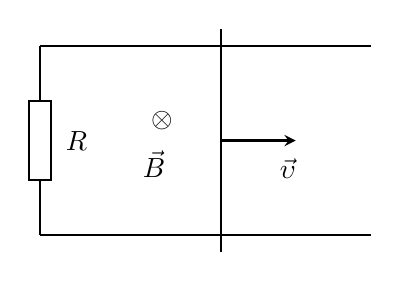
\begin{tikzpicture}[>=stealth, line width=0.8pt]
\draw (0,2.4)--(4.2,2.4);
\draw (0,0)--(4.2,0);
\draw (0,0)--(0,0.7);
\draw (0,1.7)--(0,2.4);
\draw[fill=white] (-0.14,0.7) rectangle (0.14,1.7);
\node[right] at (0.2,1.2) {$R$};
\draw (2.3,-0.22)--(2.3,2.62);
\draw[->] (2.3,1.2)--(3.25,1.2);
\node[below] at (3.15,1.1) {$\vec{\upsilon}$};
\node at (1.55,1.45) {$\otimes$};
\node[below] at (1.45,1.2) {$\vec{B}$};
\end{tikzpicture}
\end{center}
}{
\smallskip\noindent\textbf{Решение от GPT}\par
ЭДС движения равна \(\mathcal{E}=Bl\upsilon\). По закону Ома
\[
R=\frac{Bl\upsilon}{i_{\text{инд}}}=\frac{0{,}1\cdot0{,}10\cdot2}{0{,}010}=2\,\text{Ом}.
\]
Ответ: \(2\,\text{Ом}\).
}

% Source c584F9: https://ege.fipi.ru/bank/questions.php?search=1&proj=BA1F39653304A5B041B656915DC36B38&qid=c584F9
\BankTask{c584F9}{
По гладким параллельным проводящим рельсам, которые расположены на диэлектрической подножке и замкнуты на резистор $R$, перемещают лёгкий тонкий проводник $MN$. Рельсы, резистор и проводник образуют контур, который находится в однородном магнитном поле с вектором магнитной индукции $\vec{B}$, как показано на рисунке а. При движении проводника площадь, ограниченная контуром, изменяется с течением времени так, как указано на рисунке б. ЭДС самоиндукции, возникающей в контуре, пренебречь.

\begin{enumerate}
\item В интервале времени от $20$ до $40\,\text{с}$ в резисторе течёт ток.
\item Модуль ЭДС индукции, возникающей в контуре, достигает максимального значения в интервале времени от $40$ до $50\,\text{с}$.
\item В интервале времени от $0$ до $20\,\text{с}$ сила Ампера, действующая на проводник, направлена влево.
\item Величина силы, прикладываемой к проводнику для его перемещения, максимальна в интервале времени от $40$ до $50\,\text{с}$.
\item Поскольку рельсы гладкие, для перемещения проводника к нему не надо прикладывать силу ни в один из интервалов времени, представленных на графике на рис. б.
\end{enumerate}

\begin{center}
\begin{tikzpicture}[book diagram,x=0.8cm,y=0.8cm]
\draw[line width=2pt] (0,0)--(6,0) (0,1.95)--(6,1.95);
\draw (1.2,-0.4)--(1.2,2.35);
\node[above left] at (1.2,2.05) {$N$};
\node[below left] at (1.2,-0.05) {$M$};
\draw (4.8,1.95)--(4.8,1.48) (4.8,0.5)--(4.8,0);
\draw (4.53,0.5) rectangle (5.07,1.48);
\node[right] at (5.1,0.99) {$R$};
\draw (2.96,0.94) circle (0.33);
\draw (2.73,0.71)--(3.19,1.17) (2.73,1.17)--(3.19,0.71);
\node[below right] at (3.32,0.93) {$\vec B$};
\node at (3,-0.8) {Рис. а};
\end{tikzpicture}
\qquad
\begin{tikzpicture}[book diagram,x=0.052cm,y=2.7cm]
\draw[-{book tip}] (0,0)--(65,0) node[right] {$t,\,\text{с}$};
\draw[-{book tip}] (0,0)--(0,1.04) node[above left] {$S,\,\text{м}^2$};
\node[below left] at (0,0) {$0$};
\foreach \x in {10,20,30,40,50} {
\draw (\x,-0.025)--(\x,0.025);
\node[below] at (\x,-0.035) {$\x$};
}
\foreach \x in {5,15,25,35,45,55} {\draw (\x,-0.014)--(\x,0.014);}
\foreach \y/\lab in {0.2/{0{,}2},0.4/{0{,}4},0.6/{0{,}6},0.8/{0{,}8}} {
\draw (-1.3,\y)--(1.3,\y);
\node[left] at (-1.5,\y) {$\lab$};
}
\foreach \y in {0.1,0.3,0.5,0.7,0.9} {\draw (-0.7,\y)--(0.7,\y);}
\draw[thick] (0,0.2)--(20,0.8)--(40,0.8)--(50,0.2);
\draw (0,0.2)--(18,0.2) (20,0.1)--(20,0.36) (37,0.2)--(50,0.2) (40,0.44)--(40,0.8);
\node at (30,-0.31) {Рис. б};
\end{tikzpicture}
\end{center}
}{
\smallskip\noindent\textbf{Решение от GPT}\par
По закону Фарадея $|\mathcal E|=B|\Delta S/\Delta t|$: на интервалах $0$–$20$, $20$–$40$ и $40$–$50\,\text{с}$ модули скорости изменения площади равны соответственно $0{,}03$, $0$ и $0{,}06\,\text{м}^2/\text{с}$, поэтому утверждение 1 неверно, а 2 верно. В первые $20\,\text{с}$ площадь увеличивается, проводник движется влево, а сила Ампера по правилу Ленца направлена вправо: утверждение 3 неверно. При пренебрежении инерцией лёгкого проводника прикладываемая сила уравновешивает силу Ампера, $F=BIl=\frac{B^2l}{R}|dS/dt|$, поэтому утверждение 4 верно. Гладкость рельсов устраняет трение, но не магнитное торможение, поэтому утверждение 5 неверно. Ответ: 2, 4.
}

% Source 39266: https://phys-ege.sdamgia.ru/problem?id=39266
\BankTask{39266}{
\begin{center}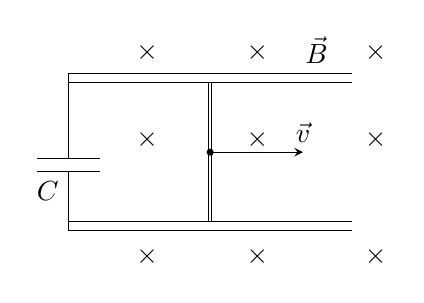
\begin{tikzpicture}[>=stealth]

\draw (0,.92)--(0,2)--(3.6,2) (0,.76)--(0,0)--(3.6,0) (-.4,.76)--(.4,.76) (-.4,.92)--(.4,.92);
\draw (0,1.88)--(3.6,1.88) (0,.12)--(3.6,.12);\draw[double] (1.8,.12)--(1.8,1.88);
\node[below left]at(0,.75){$C$};\draw[->] (1.8,1)--(2.98,1)node[above]{$\vec v$};\fill (1.8,1)circle(.045);
\foreach \x in {1,2.4,3.9}{\foreach \y in {-.32,1.16,2.26}{\node at(\x,\y){$\times$};}}
\node[above]at(3.15,2){$\vec B$};
\end{tikzpicture}\end{center}
По двум горизонтально расположенным параллельным проводящим рельсам с пренебрежимо малым сопротивлением, замкнутым на конденсатор электроёмкостью С  =  $100$ мкФ, поступательно и равномерно скользит проводящий стержень. Расстояние между рельсами l  =  $1\,\text{м}$. Рельсы со стержнем находятся в вертикальном однородном магнитном поле с индукцией B  =  $1$ Тл (см. рис.). Через достаточно большой промежуток времени от начала движения энергия электрического поля конденсатора W  =  $50$ мкДж. Какова скорость движения стержня? Рельсы закреплены на диэлектрической подложке.
}{
\smallskip\noindent\textbf{Решение}\par
$1$.  Модуль ЭДС индукции, возникающей в контуре при движении стержня: $|\mathcal E|=B v l,$где B  — модуль вектора магнитной индукции, \ensuremath{\upsilon}  — скорость движения стержня, l  — длина стержня. 
$2$.  Так как напряжение на конденсаторе $U_{c}$ равно модулю ЭДС индукции, то энергия электрического поля конденсатора определяется по формуле: 

\[W= \frac{C U_C ^2}{2} = \frac{C B ^2 v ^2 l ^2}{2} .\]

В итоге скорость стержня равна: 

\[v = \sqrt{\frac{2 W}{C B ^2 l ^2}} = \sqrt{\frac{2 \cdot 50 \cdot 10^{-6}}{100 \cdot 10 ^{ - 6 } \cdot 1 ^2 \cdot 1 ^2}} =1 \,\text{м} / \,\text{с}.\]

Ответ: $1\,\text{м/с}$.
}

\end{document}
